% ==============================================================
% 多次元 Apriori-Window: 多次元トランザクションデータにおける密集アイテムセット領域の厳密抽出
% ==============================================================
% コンパイル:
%   xelatex main.tex && bibtex main && xelatex main.tex && xelatex main.tex
% ==============================================================
\documentclass[conference]{IEEEtran}
\IEEEoverridecommandlockouts

% --- 日本語対応 ---
\usepackage{xeCJK}
\setCJKmainfont[AutoFakeBold=2.5]{Hiragino Mincho ProN}
\setCJKsansfont{Hiragino Sans}
\setCJKmonofont{Hiragino Sans}

% --- 標準パッケージ ---
\usepackage{cite}
\usepackage{amsmath,amssymb,amsfonts}
\usepackage{amsthm}
\usepackage{algorithm}
\usepackage{algpseudocode}
\usepackage{graphicx}
\usepackage{textcomp}
\usepackage{xcolor}
\usepackage{threeparttable}
\usepackage{subcaption}
\usepackage{booktabs}
\usepackage{url}
\usepackage{multirow}
\usepackage{bm}
\usepackage{tikz}
\usetikzlibrary{arrows.meta, positioning, shapes.geometric, fit}

% --- 定理環境 ---
\newtheorem{definition}{定義}
\newtheorem{theorem}{定理}
\newtheorem{lemma}{補題}
\newtheorem{remark}{注意}
\newtheorem{example}{例}

\def\BibTeX{{\rm B\kern-.05em{\sc i\kern-.025em b}\kern-.08em
    T\kern-.1667em\lower.7ex\hbox{E}\kern-.125emX}}

\begin{document}

\title{Multi-Dimensional Apriori-Window: \\
Exact Mining of Dense Itemset Regions\\
over Arbitrary Dimensions}

\author{
  \IEEEauthorblockN{1\textsuperscript{st} Given Name Surname}
  \IEEEauthorblockA{
    \textit{Dept. Name of Organization}\\
    \textit{Name of Organization}\\
    City, Country\\
    email@example.com}
  \and
  \IEEEauthorblockN{2\textsuperscript{nd} Given Name Surname}
  \IEEEauthorblockA{
    \textit{Dept. Name of Organization}\\
    \textit{Name of Organization}\\
    City, Country\\
    email@example.com}
}

\maketitle
\pagestyle{plain}
\pagenumbering{arabic}

\begin{abstract}
大規模小売・疫学・物流データでは、
\emph{何が}密集しているか（アイテムセット）と
\emph{いつ・どこで}密集しているか（時空間領域）を
同時に答えることが求められるが、
既存手法はこの両方を達成できない：
パターンマイニング系手法は領域を出力せず、
領域抽出系手法（M-Zoom 等）は
直積ブロック制約や反単調性の欠如により
アイテムセット列挙と統合できない。
本稿では、アイテムセットとそれが密集する多次元領域を厳密に抽出する
\textbf{多次元 Apriori-Window}を提案する。
固定空間開始点ごとに多次元問題を
重複時刻を許す1次元問題へ還元し、
窓内出現数の反単調性を活用した Apriori 枝刈りにより
全密集パターンとその任意形状の密集領域を厳密に列挙する。

提案手法は定義により全密集パターンとその密集領域を
厳密に抽出する（F1 $= 1.00$、Jaccard $= 1.00$）。
多様な形状の密集領域を埋め込んだ合成データでの比較実験では，
既存のパターンマイニング系手法はパターン検出F1 = 0.356--0.917と
密集領域の形状により精度にばらつきが見られた。
領域抽出系手法（MZoom・LISA・ST-DBSCAN）は
GT パターンを与えても mean Jaccard $\leq$ 0.190 に留まり，
スライディング窓定義による密集領域を精度良く近似できなかった。
スケーラビリティ実験では，
トランザクション数 $N$ を $10^3$--$10^8$ の 5 桁にわたって変化させ，
$N$ に対する線形スケーリングを確認した
（$10^8$ トランザクションを約 12 分で処理）。
さらに犯罪・苦情・地震の$d{=}3$--$4$実データへの適用により、
ドメイン知識と整合する解釈可能な示唆が得られることを確認した。
\end{abstract}

\begin{IEEEkeywords}
頻出パターンマイニング, 多次元データ, スライディングウィンドウ,
密集領域検出, Apriori, 区間表現
\end{IEEEkeywords}

% ==============================================================
\section{はじめに}\label{sec:intro}
% ==============================================================

\subsection{動機と応用背景}

大規模小売チェーンのデータアナリストは、
「どの商品の組み合わせが、どの店舗で、いつ集中的に購買されるか」
を知りたいと考える。
例えば、100 店舗 $\times$ 52 週の POS データから
「ビールとポテトチップスは週 46--52（年末商戦）の都市部店舗（店舗 0--9）で
集中購買される」という知見は、
地域特化の在庫計画やプロモーション施策に直結する。
同様に、疫学では特定地域・特定時期に集中する症状の共起パターンが
介入ターゲットとなり、
物流では地域・時間帯別の出荷量急増パターンが
サービス最適化を支援する。

このような\emph{時空間局所的な密集パターン}を発見するには、
トランザクションデータの時刻情報と空間情報
（店舗 ID・地域コード・GPS 座標等）を
同時に扱うマイニング手法が必要である。

\subsection{同時出力の必要性と既存手法の限界}

上記の応用において分析者が真に必要とする出力は、
(i)~\emph{何が}密集しているか（アイテムセット $P$）と
(ii)~\emph{いつ・どこで}密集しているか（$d$ 次元密集領域）の
組 $(P, R(P))$ である。
パターン $P$ だけでは「どの店舗にいつ追加発注すべきか」が不明であり、
領域 $R$ だけでは「何を発注すべきか」が特定できない。
両者が揃って初めて、地域・時期に特化した施策を立案できる。
しかし、既存手法はいずれもこの両方を同時に提供できない。

\paragraph{パターンマイニング系手法.}
頻出パターンマイニング~\cite{agrawal1994apriori,han2000mining}は
グローバルサポートに基づくため局所的密集パターンを見逃す。
Apriori-Window~\cite{aprioriwindow}は時間軸のみの1次元設計であり
空間情報を活用できない。
これらは「何が密集しているか」には答えられるが
「どこで密集しているか」には答えられない。

\paragraph{領域抽出系手法.}
密部分テンソルマイニング（M-Zoom~\cite{shin2018mzoom}等）は
直積ブロック制約により任意形状の密集領域にフィットできず、
パターン列挙も不正確である（\S\ref{sec:related}で詳述）。
空間統計手法~\cite{anselin1995lisa,ord1995getis}は時間次元を扱えない。
スキャン統計~\cite{kulldorff1997spatial}は単一変量限定である。
ST-DBSCAN~\cite{birant2007stdbscan}は点近傍密度に基づくため
背景密度と区別された局所的密集を検出できず、
反単調性も満たさないため Apriori 枝刈りと統合できない。

\subsection{本研究の貢献}

本稿では、Apriori-Window~\cite{aprioriwindow}を
任意の $d$ 次元グリッド
（時間 + $d{-}1$ 個の空間・カテゴリ次元）に拡張した
\textbf{多次元 Apriori-Window}を提案する（\S\ref{sec:method}）。
提案手法の特長を一言で表すと、
\textbf{アナリストが「いつ・どこで・何が売れるか」を偽陽性ゼロで抽出できる}
ことである。

本研究の技術的本質は、
1次元 Apriori-Window~\cite{aprioriwindow}の密集区間計算を、
固定空間開始点ごとの時間多重集合へ適用する形で
$d$ 次元へ拡張した点にある。
すなわち、多次元化しても本質的に解いているのは
\emph{重複を許す1次元 Apriori-Window} である。

\begin{enumerate}
\item \textbf{固定空間開始点ごとの 1D 還元}：
各空間開始点 $\bm{s}_{\mathrm{sp}}$ ごとに、
その空間窓に入るパターンの出現を時刻の多重集合
$L_P(\bm{s}_{\mathrm{sp}})$ へ潰す。
これにより $d$ 次元問題は、
空間開始点をキーとする複数の1次元問題に分解される。

\item \textbf{duplicate-aware $t$ 軸ストライド}：
2次元以上では同一時刻の重複が生じる。
1点ずつ dense start を保持するのではなく、
現在窓だけで dense が保証される left の連続ブロックをまとめて処理し、
密集区間として出力する（Lemma~\ref{lem:stride}）。

\item \textbf{singleton interval map の交差による Apriori 枝刈り}：
各アイテムの密集領域を
空間開始点ごとの時間区間列として保持し、
候補パターンではそれらを交差して候補区間を作る。
これにより $k \geq 2$ でも1次元と同型の区間ベース枝刈りが適用できる
（Lemma~\ref{lem:apriori}）。
\end{enumerate}

% ==============================================================
\section{関連研究}\label{sec:related}
% ==============================================================

本研究は、時空間トランザクションデータから
密集アイテムセット領域を発見する問題を扱う。
この問題は2つの研究系譜の交点に位置する：
(1)~アイテムセットの列挙を目的とする\emph{パターンマイニング系譜}と、
(2)~多次元空間における密集ブロックの検出を目的とする\emph{密ブロック検出系譜}である。
以下では両系譜を整理し、本研究がなぜその交点に位置するかを明確にする。

% ==============================================================
\subsection{パターンマイニング系譜}
% ==============================================================

\paragraph{頻出アイテムセットマイニング（FIM）.}
Agrawal ら~\cite{agrawal1994apriori}の Apriori アルゴリズムは、
アイテムセットの単調性（部分集合は常に親集合以上のサポートを持つ）を利用して
候補空間を大幅に枝刈りする。
Han ら~\cite{han2000mining}の FP-Growth は
接頭辞木を用いてさらに高速化する。
これらは静的なトランザクションデータベース全体の
グローバルサポートを基準とするため、
局所的に密集したパターンを見逃すという
根本的な問題を抱える~\cite{aprioriwindow}。

\paragraph{出現間隔ベースの手法（LPFIM / LPPM）.}
局所密集区間の検出を目的として、
連続する出現タイムスタンプ間の\emph{間隔}に基づく
複数の手法が提案されている。
LPFIM~\cite{mahanta2005lpfim}は
連続する2出現のギャップが閾値 minthd1 を超えた時点で区間を分割し、
局所サポート率が閾値以上かつ区間長が minthd2 以上の区間を出力する。
LPPM~\cite{fournierviger2021lppm}は
余剰累積（spillover）を導入してノイズに頑健な区間検出を実現する。

これらの手法は
「連続する2出現の時刻差（出現間隔）」を評価することで密集を推定する。
しかし、高橋ら~\cite{aprioriwindow}が指摘するように、
ギャップパラメータがパターン同定精度と区間検出精度の双方を支配するため、
両者を同時に高く保つパラメータ設定が一般に存在しない
という構造的限界を持つ。

さらに、これらの手法は\emph{本質的に多次元への拡張が不可能}である。
$d$ 次元グリッド上の出現点集合には線形順序が存在せず、
「連続する2出現の間隔」が定義できないためである。

\paragraph{Apriori-Window（直接の前身研究）.}
Apriori-Window~\cite{aprioriwindow}は
この構造的限界を解消する厳密解法である。
出現間隔を介さず、スライディング窓 $[l, l+W]$ 内の出現数を\emph{直接}計算することで
局所頻度を評価するため、ギャップパラメータを必要としない。
反単調性に基づく Apriori 枝刈りと $t$ 軸ストライドにより、
密集区間を網羅的かつ厳密に列挙する。
比較実験では LPFIM・LPPM を大幅に上回る性能を示した~\cite{aprioriwindow}。

\emph{多次元化が可能な理由}：
「矩形窓内の出現数」という定義は $d$ 次元でも自然に拡張できる
（窓を $d$ 次元直方体 $\prod_k [s_k, s_k+W_k]$ に置き換えるだけ）。
出現間隔ベースの手法が線形順序に依存するのと対照的に、
Apriori-Window の設計は線形順序を必要としない。
本研究はこの観察に基づき、
Apriori-Window を1次元から任意の $d$ 次元へ拡張する。

\paragraph{コロケーションマイニング.}
コロケーションマイニング~\cite{shekhar2001colocation}は、
複数種のフィーチャーが地理的近傍に共存するパターンを
参加指数（PI）で評価する。
Qian ら~\cite{qian2009stcolocation}はこれを
重み付きスライディングウィンドウに拡張した（STCP-Miner）。
これらはトランザクション単位の共起ではなく
空間的近傍に基づく共起を扱い、
密集領域の抽出は対象としない。
ただし、パターン識別精度（F1）の観点では比較が可能である（\S\ref{sec:ex1_1}）。

% ==============================================================
\subsection{領域抽出系譜}
% ==============================================================

パターンマイニング系譜が「何が密集しているか」に答える手法群であるのに対し、
以下の手法群は「どこで密集しているか」に答えることを目的とする。
しかし後述するように、
いずれも効率的なアイテムセット列挙と両立させることができない。

% --- 密部分テンソルマイニング ---
\paragraph{密部分テンソルマイニング.}
M-Zoom~\cite{shin2018mzoom}をはじめとする
密部分テンソル手法群~\cite{jiang2015crossspot,shin2018mbiz,shin2017dcube,feng2020specgreedy,shin2017densealert,shin2023catchcore}は、
多次元テンソルにおける密ブロックを検出する。
各次元で値の集合 $B_k \subseteq D_k$ を選択し、
直積ブロック $\prod_k B_k$ の質量/体積比を最大化する
グリーディ探索を行う。

これらの手法には2つの構造的限界がある。

\emph{第一に、出力が直積ブロックに限定される。}
不規則な形状の密集領域に対しては、
過剰な領域を含むか密集セルを取りこぼすかが不可避であり、
GT パターンを与えても Jaccard が低下する
（\S\ref{sec:ex1_1}で実証）。

\emph{第二に、パターン列挙が不正確である。}
アイテムを追加次元として含めれば列挙は試みられるが、
直積制約によりブロック内のアイテム集合 $C_B$ の全部分集合が
同一領域で密集と仮定され、偽陽性が生じる（\S\ref{sec:ex1_1}で実証）。
異なるパターンの密集領域を区別することもできない。
これは反単調性に基づく Apriori 枝刈りとは根本的に異なる
貪欲探索であり、体系的なパターン列挙機構を持たない。

% --- 空間統計手法 ---
\paragraph{空間統計手法.}
LISA~\cite{anselin1995lisa}は局所 Moran's $I$ で空間ホットスポットを同定し、
Getis-Ord $G_i^*$~\cite{ord1995getis}は
局所集中度を $z$ スコアで評価する。
いずれも\emph{空間次元のみ}が対象であり、
時間スライスごとの個別実行では時間的連続性が失われる。

% --- 空間・時空間スキャン統計 ---
\paragraph{空間・時空間スキャン統計.}
Kulldorff~\cite{kulldorff1997spatial,kulldorff2001prospective}の
空間/時空間スキャン統計は、
円形・円柱形の走査窓で有意なクラスタを検出する。
FlexScan~\cite{tango2005flexscan}は
不整形窓への拡張を行った。

上記の統計手法はいずれも\emph{単一変量}の異常集中を検出する設計であり、
アイテムセットの概念を持たない。
全パターンの列挙には $O(2^{|\mathcal{I}|})$ 回の独立実行が必要であり、
Apriori 枝刈りとの統合は設計されていない。

% --- 時空間クラスタリング ---
\paragraph{時空間密度ベースクラスタリング（ST-DBSCAN 等）.}
ST-DBSCAN~\cite{birant2007stdbscan}は
DBSCAN~\cite{ester1996dbscan}を時空間データに拡張し、
空間的距離と時間的距離にそれぞれ独立な閾値
$\varepsilon_1, \varepsilon_2$ を設ける。
任意形状のクラスタを出力できるが、
2つの根本的な差異が残る。
第一に、点近傍のカウントにより密度を定義するため、
出現が空間的に均一な場合にはデータ全体が単一クラスタとなり、
局所的密集を識別できない。
本手法は窓内出現数と絶対閾値 $\theta$ により
背景密度と区別された局所的密集を検出する。
第二に、点近傍密度は反単調性を持たないため、
全パターンの独立処理 $O(2^{|\mathcal{I}|})$ が不可避である。

上記の領域抽出系手法はいずれもアイテムセットの概念を持たないが、
GT パターンとその出現密度を与えれば
領域抽出器として評価が可能である（\S\ref{sec:ex1_1}）。

% ==============================================================
\subsection{本研究の位置づけ}
% ==============================================================

以上の分析により、既存手法はいずれも
パターン列挙と多次元密集領域抽出を同時に達成できないことが示された。
本研究は窓内出現数に基づく密集定義の反単調性を利用して
Apriori 枝刈りを自然に統合し、
両者を単一のフレームワークで実現する。
表~\ref{tab:related}にこの位置づけを示す。

\begin{table}[t]
\centering
\caption{関連手法との比較。
「アイテムセット」はパターン列挙能力、
「密集領域」は時空間的に局所化された密集領域の出力能力を指す。}
\label{tab:related}
\small
\begin{tabular}{lccc}
\toprule
手法 & \shortstack{アイテム\\セット} & \shortstack{時空間\\密集領域} & \shortstack{領域\\形状} \\
\midrule
Apriori~\cite{agrawal1994apriori}
                                          & $\checkmark$ & $\times$     & ---          \\
LPFIM~\cite{mahanta2005lpfim} / LPPM~\cite{fournierviger2021lppm}
                                          & $\checkmark$ & 1Dのみ      & 区間     \\
Apriori-Window~\cite{aprioriwindow}       & $\checkmark$ & 1Dのみ      & 区間     \\
コロケーション~\cite{shekhar2001colocation}
                                          & $\checkmark$ & $\times$     & ---          \\
STCP-Miner~\cite{qian2009stcolocation}   & $\checkmark$ & $\times$     & ---          \\
\midrule
M-Zoom~\cite{shin2018mzoom} 他           & $\triangle$$^*$     & $\checkmark$ & 直積のみ \\
SaTScan~\cite{kulldorff1997spatial}       & $\times$     & $\checkmark$ & 円/円柱 \\
FlexScan~\cite{tango2005flexscan}        & $\times$     & $\checkmark$ & 不整形    \\
LISA~\cite{anselin1995lisa}
  / $G_i^*$~\cite{ord1995getis}          & $\times$     & 空間のみ     & 任意         \\
ST-DBSCAN~\cite{birant2007stdbscan} 等   & $\times$   & $\checkmark$ & 任意    \\
\midrule
\textbf{本手法}                              & $\checkmark$ & $\checkmark$ & 任意    \\
\bottomrule
\multicolumn{4}{l}{\scriptsize $^*$アイテムを次元に含めればパターン出力は可能だが、} \\
\multicolumn{4}{l}{\scriptsize \hspace{1em}直積制約により偽陽性が生じ領域分離も不可能。}
\end{tabular}
\end{table}

% ==============================================================
\section{問題定義}\label{sec:problem}
% ==============================================================

本節では、Apriori-Window~\cite{aprioriwindow} の1次元設定を復習し（\S\ref{sec:1d_review}）、
続いてその $d$ 次元拡張を定式化する（\S\ref{sec:nd_extension}）。

% ==============================================================
\subsection{Apriori-Window（1次元）}\label{sec:1d_review}
% ==============================================================

$\mathcal{I} = \{i_1, \ldots, i_m\}$ をアイテム全体集合、
$\mathcal{D}_{\mathrm{1D}} = \{(t_n, d_n)\}_{n=1}^N$ を
タイムスタンプ付きトランザクション列とする。
ここで $t_n \in \mathbb{Z}_{\geq 0}$ は整数タイムスタンプ、
$d_n \subseteq \mathcal{I}$ はアイテム集合である。

パターン $P \subseteq \mathcal{I}$ の出現列を
\[
  \mathrm{occ}(P) = \{t_n : P \subseteq d_n\}
\]
とする。

\begin{definition}[区間サポート~\cite{aprioriwindow}]\label{def:sup1d}
ウィンドウ幅 $W$（$W > 0$）のもとで、
ウィンドウ左端 $l$ に対するパターン $P$ の区間サポートを
\[
  \mathrm{sup}(P,\, l,\, W)
  = \bigl|\{t \in \mathrm{occ}(P) : l \leq t \leq l + W\}\bigr|
\]
と定義する。窓 $[l, l+W]$ は $W+1$ 個の離散時刻を含む。
\end{definition}

\begin{definition}[密集開始点集合と密集区間]\label{def:dense1d}
サポート閾値 $\theta$ に対し、
\[
  \mathcal{T}_\theta(P)
  = \{l \in \mathbb{Z}_{\geq 0} : \mathrm{sup}(P, l, W) \geq \theta\}
\]
を $P$ の\emph{密集開始点集合}とする。

$[a,b] \subseteq \mathcal{T}_\theta(P)$ を最大連続成分とする。
このとき $[a,\, b + W]$ を $P$ の\emph{密集区間}と呼ぶ。
\end{definition}


% ==============================================================
\subsection{$d$ 次元への拡張}\label{sec:nd_extension}
% ==============================================================

$\mathcal{D} = \{(\bm{b}_n, d_n)\}_{n=1}^N$ を
$d$ 次元トランザクション列とする。ここで
\[
  \bm{b}_n = (b_n^{(0)}, b_n^{(1)}, \ldots, b_n^{(d-1)})
  \in \prod_{k=0}^{d-1}\{0,1,\ldots,N_k-1\}
\]
は整数座標ベクトル（第0軸は時間）、
$d_n \subseteq \mathcal{I}$ はアイテム集合である。
$N$ は\emph{トランザクション数}を表す。

\begin{definition}[固定空間開始点への時間多重集合還元]\label{def:collapsed_multiset_nd}
空間開始ベクトル
\[
  \bm{s}_{\mathrm{sp}} = (s_1, \ldots, s_{d-1})
\]
と空間ウィンドウ幅
$\bm{W}_{\mathrm{sp}} = (W_1, \ldots, W_{d-1})$
（各 $W_k > 0$）を固定する。
軸 $k$ の空間窓 $[s_k, s_k + W_k]$ は $W_k + 1$ 個の離散座標を含む。
パターン $P$ の時間多重集合を
\[
  L_P(\bm{s}_{\mathrm{sp}})
  =
  \{\!\{
    b_n^{(0)}
    \mid
    P \subseteq d_n,\;
    s_k \leq b_n^{(k)} \leq s_k + W_k\; (\forall k=1,\ldots,d-1)
  \}\!\}
\]
と定義する。ここで $\{\!\{\cdot\}\!\}$ は重複を許す多重集合を表す。
\end{definition}

この定義の本質は、固定空間開始点ごとに
$d$ 次元問題を\emph{重複タイムスタンプを許す1次元問題}へ還元することにある。

\begin{definition}[$d$ 次元スライディングウィンドウサポート]\label{def:support_nd}
時間開始点 $s_0$ と空間開始ベクトル $\bm{s}_{\mathrm{sp}}$ に対し、
パターン $P$ のサポートを
\begin{equation}\label{eq:support_nd}
  S_P(s_0, \bm{s}_{\mathrm{sp}})
  = \bigl|\{t \in L_P(\bm{s}_{\mathrm{sp}}) : s_0 \leq t \leq s_0 + W_0\}\bigr|
\end{equation}
と定義する。
\end{definition}

\begin{definition}[密集開始点集合と密集領域]\label{def:dense_region_nd}
固定空間開始ベクトル $\bm{s}_{\mathrm{sp}}$ に対し、
\[
  \mathcal{T}_\theta(P,\bm{s}_{\mathrm{sp}})
  =
  \{s_0 \in \mathbb{Z}_{\geq 0} : S_P(s_0,\bm{s}_{\mathrm{sp}}) \geq \theta\}
\]
を空間開始点 $\bm{s}_{\mathrm{sp}}$ における $P$ の\emph{密集開始点集合}とする。

$[a_j,b_j]$ を $\mathcal{T}_\theta(P,\bm{s}_{\mathrm{sp}})$ の最大連続成分とする。
このとき $[a_j,\, b_j + W_0]$ を空間開始点 $\bm{s}_{\mathrm{sp}}$ における
$P$ の\emph{密集区間}と呼ぶ
（定義~\ref{def:dense1d} の自然な拡張）。

全空間開始点にわたる密集区間の集合
\[
  \mathcal{R}_\theta(P)
  = \{(\bm{s}_{\mathrm{sp}},\, [a_j,\, b_j + W_0])\}
\]
を $P$ の\emph{密集領域}と呼ぶ。
\end{definition}

\paragraph{Apriori 単調性.}

\begin{lemma}[密集開始点集合の単調性]\label{lem:apriori}
任意のパターン $P$ とその部分集合 $Q \subset P$、
任意の空間開始ベクトル $\bm{s}_{\mathrm{sp}}$ に対して、
\[
  \mathcal{T}_\theta(P,\bm{s}_{\mathrm{sp}})
  \subseteq
  \mathcal{T}_\theta(Q,\bm{s}_{\mathrm{sp}})
\]
が成立する。
\end{lemma}

証明は付録~\ref{sec:proofs}に示す。

補題~\ref{lem:apriori} より、パターン $P$ の密集開始点集合は
各 singleton item $i \in P$ の密集区間に包含される。
提案手法ではこの性質を用いて、
\emph{singleton interval map の交差}を候補区間として利用する（\S\ref{sec:alg_k2}）。

\subsection{$d$ 次元密集領域検出問題}\label{sec:dense_detection}

$d$ 次元密集領域検出問題とは、
$d$ 次元トランザクション列 $\mathcal{D}$、
ウィンドウ幅
$\bm{W} = (W_0, W_1, \ldots, W_{d-1}) \in \mathbb{Z}_{>0}^d$、
サポート閾値 $\theta$ が与えられたとき、
各パターン $P$ に対する密集領域の完全な集合
$\mathcal{R}_\theta(P)
= \{(\bm{s}_{\mathrm{sp}}, [a_j,\, b_j + W_0])\}$
を求める問題である。
各軸 $k$ の窓は閉区間 $[s_k, s_k + W_k]$（$W_k + 1$ ビン）である。

% ==============================================================
\section{提案手法：多次元 Apriori-Window アルゴリズム}
\label{sec:method}
% ==============================================================

\S\ref{sec:dense_detection} の問題を解くための
\textbf{多次元 Apriori-Window アルゴリズム}を提案する。
現在の実装は密集開始点集合やサポートサーフェスを明示的に構築しない。
その代わり、各固定空間開始点に対して
\emph{重複考慮1次元 Apriori-Window} を解き、
出力を密集領域として保持する。

% ==============================================================
\subsection{固定空間開始点による1次元多重集合還元}\label{sec:binsearch}
% ==============================================================

パターン $P$ と固定空間開始点 $\bm{s}_{\mathrm{sp}}$ に対し、
定義~\ref{def:collapsed_multiset_nd} の時間多重集合
$L_P(\bm{s}_{\mathrm{sp}})$ を構築する。
これは $P$ の各出現トランザクションを、
そのトランザクションを含みうるすべての空間開始点へ配布することで得られる。

\paragraph{空間開始点への配布.}
パターン $P$ を含むトランザクションが離散座標
\[
  \bm{b} = (b^{(0)}, b^{(1)}, \ldots, b^{(d-1)})
\]
にあるとき、そのトランザクションを含む空間開始点の第 $k$ 成分（$k \geq 1$）は
\[
  s_k \in [\max(0,\, b^{(k)} - W_k),\; b^{(k)}]
\]
を満たす。したがって1つの出現は高々
\[
  W_{\mathrm{sp}} = \prod_{k=1}^{d-1} (W_k + 1)
\]
個の空間開始点へ寄与する。

\paragraph{構築コスト.}
パターン $P$ の出現トランザクション数を $N_P$ とする。
構築には $O(N_P \cdot W_{\mathrm{sp}})$ を要し、
ソートを含めた総計算量は $O(\widetilde N_P \log \widetilde N_P)$ である。
ただし $\widetilde N_P = N_P \cdot W_{\mathrm{sp}}$ とする。

% ==============================================================
\subsection{$t$ 軸上の重複考慮区間ソルバー}\label{sec:t_stride}
% ==============================================================

固定空間開始点 $\bm{s}_{\mathrm{sp}}$ に対し、
ソート済み多重集合 $L = L_P(\bm{s}_{\mathrm{sp}})$ を考える。
ここで重要なのは、2次元以上では同じタイムスタンプが複数回出現しうることである。
このため、1次元の単純な ``$+1$ ジャンプ'' をそのまま使うのではなく、
\emph{現在の窓だけで密集が保証される左端の連続ブロック}を一括処理する。

\paragraph{$c < \theta$ のときのジャンプ.}
現在の時間左端を $l$、窓内カウントを $c$ とする。
$c < \theta$ のとき、新しいイベントが窓へ入り始める最小の左端まで飛ぶことができる：
\begin{equation}\label{eq:jump_empty}
  l \leftarrow \max(l+1,\; L[\mathrm{next}] - W_0)
\end{equation}
ここで $L[\mathrm{next}]$ は現在窓の右境界外にある最初のイベントである。

\paragraph{$c \geq \theta$ のときの密集ブロック.}
$l_{\mathrm{lo}}$ を $L$ 中で $\geq l$ となる最初の位置、
$c$ を現在窓内のイベント数とする。
余剰 $\mathrm{surplus} = c - \theta \geq 0$ に対して、
\begin{equation}\label{eq:jump_dense}
  l_{\mathrm{dense}}
  = L[l_{\mathrm{lo}} + \mathrm{surplus}]
\end{equation}
と定める。このとき $[l,\, l_{\mathrm{dense}}]$ のすべての左端は密集である。
よって現在の窓は密集開始点の連続ブロック
\[
  [l,\, l_{\mathrm{dense}}]
\]
を一括で処理していることになる。

このブロックに対する密集区間の右端は
\[
  r_{\mathrm{block}}
  = l_{\mathrm{dense}} + W_0
\]
である（定義~\ref{def:dense_region_nd}）。
したがって現在の出力区間を $r_{\mathrm{block}}$ まで延長し、
\[
  l \leftarrow l_{\mathrm{dense}} + 1
\]
と更新する。

\begin{lemma}[密集ブロックの正確性]\label{lem:stride}
式~\eqref{eq:jump_dense} で定めた $l_{\mathrm{dense}}$ に対し、
任意の $l' \in [l,\, l_{\mathrm{dense}}]$ について
\[
  |\{t \in L : l' \leq t \leq l' + W_0\}| \geq \theta
\]
が成り立つ。
\end{lemma}

証明は付録~\ref{sec:proofs}に示す。


\begin{algorithm}[t]
\caption{固定空間開始点に対する重複考慮密集区間計算}
\label{alg:t_stride}
\begin{algorithmic}[1]
\Require ソート済み多重集合 $L$、時間窓幅 $W_0$、閾値 $\theta$
\Ensure 密集区間列 $\mathcal{R}$
\State $\mathcal{R} \leftarrow \emptyset$
\State $l \leftarrow \max(0,\, L[\theta-1] - W_0)$
\State $\mathit{open} \leftarrow \mathrm{false}$
\While{$l \leq L[\mathrm{last}]$}
  \State $l_{\mathrm{lo}} \leftarrow \mathrm{lower\_bound}(L, l)$
  \State $l_{\mathrm{hi}} \leftarrow \mathrm{upper\_bound}(L, l + W_0)$
  \State $c \leftarrow l_{\mathrm{hi}} - l_{\mathrm{lo}}$
  \If{$c < \theta$}
    \If{$\mathit{open}$}
      \State 現在の区間を $\mathcal{R}$ に追加
      \State $\mathit{open} \leftarrow \mathrm{false}$
    \EndIf
    \If{$l_{\mathrm{hi}} = |L|$} \textbf{break} \EndIf
    \State $l \leftarrow \max(l+1,\; L[l_{\mathrm{hi}}] - W_0)$
           \Comment{式~\eqref{eq:jump_empty}}
  \Else
    \State $l_{\mathrm{dense}} \leftarrow L[l_{\mathrm{lo}} + (c-\theta)]$
           \Comment{式~\eqref{eq:jump_dense}}
    \State $r_{\mathrm{block}} \leftarrow l_{\mathrm{dense}} + W_0$
    \State 現在の区間を $(l, r_{\mathrm{block}})$ で開始または延長
    \State $\mathit{open} \leftarrow \mathrm{true}$
    \State $l \leftarrow l_{\mathrm{dense}} + 1$
  \EndIf
\EndWhile
\If{$\mathit{open}$}
  \State 現在の区間を $\mathcal{R}$ に追加
\EndIf
\State \Return $\mathcal{R}$
\end{algorithmic}
\end{algorithm}

% ==============================================================
\subsection{Apriori 枝刈りによる候補区間制限（$k \geq 2$）}\label{sec:alg_k2}
% ==============================================================

補題~\ref{lem:apriori} を各 singleton item に適用すると、
パターン $P$ の任意の密集開始成分は
各 item $i \in P$ の密集区間に含まれる。
この性質を用いて、候補パターン $P$ には
\emph{singleton interval map の交差}のみを使用する。

\paragraph{候補 interval map.}
singleton item $i$ の密集領域を
\[
  \mathcal{R}_\theta(\{i\})
  = \{(\bm{s}_{\mathrm{sp}}, [a,e])\}
\]
とする。
同じ空間開始点 $\bm{s}_{\mathrm{sp}}$ に属する時間区間列を
$\mathcal{R}_\theta(\{i\})[\bm{s}_{\mathrm{sp}}]$ と書く。
候補パターン $P$ の候補 interval map を
\begin{equation}\label{eq:candidate_cells}
  \mathcal{C}(P,\bm{s}_{\mathrm{sp}})
  =
  \bigcap_{i \in P}
  \mathcal{R}_\theta(\{i\})[\bm{s}_{\mathrm{sp}}]
\end{equation}
と定義する。

ここでの交差は時間区間に対する標準的な区間交差である。
すべての空間開始点で $\mathcal{C}(P,\bm{s}_{\mathrm{sp}})=\emptyset$
ならば、$P$ は密集区間を持ちえないため枝刈りされる。

\paragraph{厳密再評価.}
$\mathcal{C}(P,\bm{s}_{\mathrm{sp}}) \neq \emptyset$ の場合にのみ、
トランザクション列を1回走査して $L_P(\bm{s}_{\mathrm{sp}})$ を構築し、
Algorithm~\ref{alg:t_stride} の候補区間版を
$\mathcal{C}(P,\bm{s}_{\mathrm{sp}})$ に対して実行する。

% ==============================================================
\subsection{アルゴリズム全体と計算量}\label{sec:complexity}
% ==============================================================

\begin{algorithm}[t]
\caption{多次元 Apriori-Window（区間ベース実装）}
\label{alg:md_apriori}
\begin{algorithmic}[1]
\Require $d$ 次元トランザクション列 $\mathcal{D}$、$(\bm{W}, \theta)$
\Ensure 各パターン $P$ の密集領域 $\mathcal{R}_\theta(P)$
\ForAll{$i \in \mathcal{I}$}
  \State $L_i(\bm{s}_{\mathrm{sp}}) \leftarrow$ 空間開始点ごとの時間多重集合を構築
  \State $\mathcal{R}_\theta(\{i\}) \leftarrow$ 各 $\bm{s}_{\mathrm{sp}}$ で Algorithm~\ref{alg:t_stride} を実行
\EndFor
\State $\mathcal{F}_1 \leftarrow \{\{i\} : \mathcal{R}_\theta(\{i\}) \neq \emptyset\}$
\State $k \leftarrow 2$
\While{$\mathcal{F}_{k-1} \neq \emptyset$}
  \State \texttt{cands} $\leftarrow$ \Call{GenerateCandidates}{$\mathcal{F}_{k-1}$}
  \State \texttt{cands} $\leftarrow$ \Call{PruneCandidates}{\texttt{cands}, $\mathcal{F}_{k-1}$}
  \State $\mathcal{F}_k \leftarrow \emptyset$
  \ForAll{$P \in$ \texttt{cands}}
    \State $\mathcal{C}(P,\bm{s}_{\mathrm{sp}}) \leftarrow \bigcap_{i \in P}\mathcal{R}_\theta(\{i\})[\bm{s}_{\mathrm{sp}}]$
           \Comment{式~\eqref{eq:candidate_cells}}
    \If{すべての $\bm{s}_{\mathrm{sp}}$ で $\mathcal{C}(P,\bm{s}_{\mathrm{sp}})=\emptyset$}
      \State \textbf{continue}
    \EndIf
    \State $L_P(\bm{s}_{\mathrm{sp}}) \leftarrow$ パターン $P$ の時間多重集合を構築
    \State $\mathcal{R}_\theta(P) \leftarrow$ 各 $\bm{s}_{\mathrm{sp}}$ で候補区間版重複考慮ソルバーを実行
    \If{$\mathcal{R}_\theta(P) \neq \emptyset$}
      \State $\mathcal{F}_k \leftarrow \mathcal{F}_k \cup \{P\}$
    \EndIf
  \EndFor
  \State $k \leftarrow k + 1$
\EndWhile
\State \Return $\{\mathcal{R}_\theta(P)\}$
\end{algorithmic}
\end{algorithm}

\begin{table}[t]
\centering
\caption{提案手法の計算量。
$N_P$: パターン $P$ を含むトランザクション数、
$W_{\mathrm{sp}} = \prod_{k=1}^{d-1} (W_k + 1)$、
$\widetilde N_P = N_P W_{\mathrm{sp}}$、
$I_P$: 候補 interval map の総区間数。}
\label{tab:complexity}
\small
\begin{tabular}{lll}
\toprule
ステップ & 計算量 \\
\midrule
$L_P$ の構築 & $O(N_P \cdot W_{\mathrm{sp}})$ \\
$L_P$ のソート & $O(\widetilde N_P \log \widetilde N_P)$ \\
時間区間計算 & $O\!\left(\sum_{\bm{s}_{\mathrm{sp}}}|L_P(\bm{s}_{\mathrm{sp}})| \log |L_P(\bm{s}_{\mathrm{sp}})|\right)$ \\
候補 interval map 交差 & $O(I_P)$ \\
\bottomrule
\end{tabular}
\end{table}

したがって、現行実装に忠実な全体計算量は
\[
  O\!\left(
    \sum_{P \in \mathcal{F}}
      \bigl(
        N_P W_{\mathrm{sp}}
        +
        \widetilde N_P \log \widetilde N_P
        +
        I_P
      \bigr)
  \right)
\]
である。ここで $\mathcal{F}$ は実際に評価された候補パターンの集合である。
実データへの適用時には、連続座標の離散化が前処理として必要となる（\S\ref{sec:experiments}）。

% ==============================================================
\section{実験}\label{sec:experiments}
% ==============================================================

提案手法の有効性とスケーラビリティを検証する。
全実験はRust（リリースビルド）で実装し、
Apple M3（8コア、24\,GB RAM）上で実行した。

% ==============================================================
\subsection{EX-1：既存手法による密集領域の近似可能性}
\label{sec:ex1}\label{sec:ex1_1}
% ==============================================================

\paragraph{目的.}
\S\ref{sec:dense_detection}で定義した密集領域は
定義から一意に定まる厳密解であり、
提案手法はそれを計算する手段である。
本実験は提案手法と既存手法の精度競争ではなく、
既存手法がこの厳密解をどの程度近似できるかを評価し、
専用手法の必要性を検証するものである。

\paragraph{データ.}
4つの実データセットを使用した
（詳細はAppendix~\ref{sec:dataset_details}）。
Chicago Crime~\cite{chicagocrime}および
NYPD Crime~\cite{nypdcrime}は都市犯罪ドメイン、
NYC 311~\cite{nyc311}は市民苦情ドメイン、
USGS Earthquake~\cite{usgseq}は自然科学ドメインを代表し、
問題設定のドメイン横断的な汎用性を示す。
各データセットの生データは1イベントにつき1アイテム
（犯罪種別、苦情種別等）を含む。
連続座標（緯度、経度等）を等幅ビンに離散化してグリッドを構成し、
同一セルに属するイベントのアイテムを
1つのトランザクションに集約した
（1セル＝複数アイテムからなる1トランザクション；
グリッド構成の詳細はAppendix~\ref{sec:dataset_details}）。

\paragraph{比較手法.}
以下の手法を比較した。
パターンマイニング手法（Colocation / STCP-Miner）は
EX-1-1（密集パターン比較）のみに参加する。
領域抽出手法（MZoom / LISA / ST-DBSCAN）は
EX-1-2（密集領域比較）のみに参加し、
GTパターンを入力として与える。

\begin{itemize}
\item \textbf{Colocation}~\cite{shekhar2001colocation}: 空間コロケーションマイニング。PI閾値$\tau$をグリッドサーチ。
\item \textbf{STCP-Miner}~\cite{qian2009stcolocation}: Colocationの時空間ウィンドウ拡張。$\tau$およびウィンドウ幅をグリッドサーチ。
\item \textbf{MZoom}~\cite{shin2018mzoom}: GTパターン$P$の$d$次元出現テンソルに対する貪欲密集ブロック検出。Top $k$をグリッドサーチ。
\item \textbf{LISA}~\cite{anselin1995lisa}: GTパターン$P$の出現回数を空間グリッド上に集約し、Local Moran's $I$でHigh-Highセルを特定。
\item \textbf{ST-DBSCAN}~\cite{birant2007stdbscan}: GTパターン$P$の$d$次元出現セルに対し$\varepsilon_1$、$\varepsilon_2$、min\_ptsをグリッドサーチ。
\end{itemize}

\noindent 各比較手法のパラメータはグリッドサーチにより決定した
（詳細はAppendix~\ref{sec:grid_search_params_r1}）。
パターンマイニング手法はF1を最大化し、
領域抽出手法は平均Jaccardを最大化する設定を採用した。

\paragraph{評価指標.}
定義3--5に基づき、厳密パターン集合$P^*$および密集セル集合$R^*(P)$をGTとする。
パターンマイニング手法はF1
$= 2|\hat{P} \cap P^*| / (|\hat{P}| + |P^*|)$で評価し、
領域抽出手法はGTパターンを与えた上で
平均Jaccard $= \frac{1}{|P^*|}\sum_{P \in P^*} |R^*(P) \cap \hat{R}(P)| / |R^*(P) \cup \hat{R}(P)|$で評価する。

\paragraph{提案手法のパラメータ.}
全データセット共通：
時間ウィンドウ$W_0 = 53$（54週$\approx$1年）、
空間軸$W_k = 4$（5ビン、$k \geq 1$）。
閾値$\theta$はデータセットごとに
抽出パターン数が数十程度となるよう調整した
（Chicago: $\theta = 1{,}000$、NYPD: $\theta = 1{,}500$、
NYC 311: $\theta = 3{,}000$、USGS EQ: $\theta = 10$）。
最大パターン長は$|P| \leq 3$とした。

\paragraph{結果.}
Figure~\ref{fig:ex1_heatmap}に最良パラメータでの結果を示す。

\begin{figure}[t]
\centering
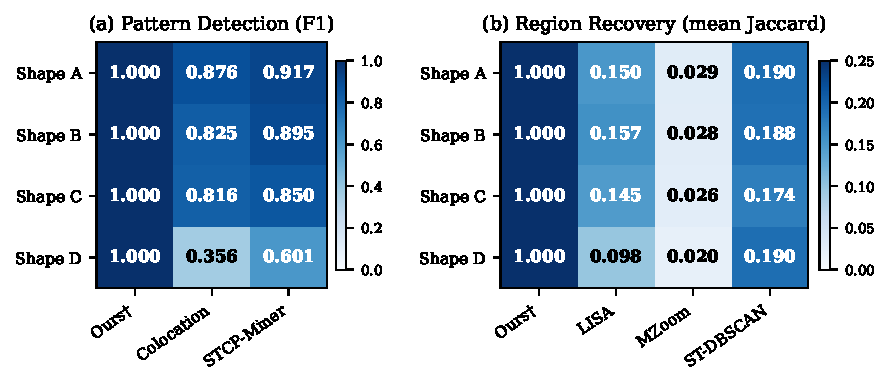
\includegraphics[width=\columnwidth]{fig/fig_ex1_heatmap.pdf}
\caption{EX-1の結果。
(a) パターン検出精度（F1）：パターンマイニング手法の最良パラメータでの結果。
(b) 領域復元精度（平均Jaccard）：GTパターンを与えた領域抽出手法の最良パラメータでの結果。
GTは定義3--5に基づく厳密解である。}
\label{fig:ex1_heatmap}
\end{figure}

\paragraph{分析.}
\emph{パターン検出精度（F1）。}
ColocationのグローバルPIは希釈の影響を受け、F1は0.26--0.69にとどまる。
STCP-Minerは時間ウィンドウにより改善するが、F1 $\leq$ 0.71に留まる。
いずれの手法も密集領域を出力しない。

\emph{領域復元精度（平均Jaccard）。}
MZoomは0.008--0.104、LISAは0.005--0.029、ST-DBSCANは0.007--0.027であり、
全データセットで0.11を下回る。
これは各手法の密度定義
（直積ブロック、時間集約、点近傍密度）が
スライディングウィンドウに基づく定義と構造的に異なるためである。
4次元データ（USGS EQ）でも同様の傾向が確認された。

% ==============================================================
\subsection{EX-2：スケーラビリティ（合成データ）}
\label{sec:ex2}
% ==============================================================

\paragraph{目的.}
提案手法の計算時間がトランザクション数$N$の増加に対して
どのようにスケールするか、
また同一$N$において時間軸長$T$と空間幅$s$の比率が
性能に影響するかを検証する。

\paragraph{合成データ生成.}
$d = 2$の格子
$\{0,\ldots,T{-}1\} \times \{0,\ldots,s{-}1\}$上で、
各アイテムを全セルに対して独立に
Bernoulli$(p_{\mathrm{item}}{=}0.10)$からサンプリングし、
1バスケットを構成する。
空セルにはデフォルトでアイテム1を割り当て、
各セルに正確に1トランザクションが存在することを保証するため、
$N = T \times s$となる
（生成の詳細はAppendix~\ref{sec:ex2_data_details}）。
$|\mathcal{I}| = 20$、$W = (24, 4)$、$\theta = 15$を固定した。

\paragraph{実験軸の選定根拠.}
$|\mathcal{I}|$および$p_{\mathrm{item}}$に対する線形スケーリングは
1次元版~\cite{aprioriwindow}で確認済みであり、
$d$の影響は$N = T \times s^{d-1}$に吸収される。
そのため$d = 2$を固定し、$T$と$s$の制御により$N$スケーラビリティを検証する。

\paragraph{実験設計.}
$T \in \{100,\; 1{,}000,\; 10{,}000,\; 100{,}000\}$および
$s \in \{10,\; 100,\; 1{,}000,\; 10{,}000\}$
の$4 \times 4 = 16$構成とした。
$N = T \times s$は$1{,}000$（$T{=}100, s{=}10$）から
$10^9$（$T{=}100{,}000, s{=}10{,}000$）の範囲をカバーする。
同一$N$で$T/s$比率が異なる構成が含まれるため、
時間軸長と空間幅が性能に与える影響を独立に観察できる。

\paragraph{結果.}
Table~\ref{tab:ex2_grid}に実行時間を示す。

\paragraph{分析.}
$N = 10^3$で0.009秒、$N = 10^8$で587--643秒であり、
$N$の$10^5$倍の増加に対して
実行時間の増加は約$6.5 \times 10^4$倍にとどまる。
$N = 10^9$は1{,}000秒以内に完了しなかった（タイムアウト）。

同一$N$でも$T/s$比率により差異が生じる：
$N = 10^7$において$T{=}100{,}000, s{=}100$は53.1\,sであるのに対し、
$T{=}1{,}000, s{=}10{,}000$は64.9\,s（1.22倍）である。
$T$が大きいほど$t$軸ストライド（Lemma~\ref{lem:stride}）による
ギャップスキップが有効に働き、
$s$が大きいほど空間始点数が増加するためである。

全体として実行時間は$N$に対しておおむね線形にスケールし、
$10^8$トランザクションを10分以内に処理可能である。

\begin{table}[t]
\centering
\caption{EX-2：2Dスケーラビリティ。
  全セルBernoulli背景のみ（埋め込みパターンなし）、
  $N = T \times s$、$\theta = 15$、$W = (24, 4)$。
  実行時間（秒）。$N = 10^9$は1{,}000\,s以内に完了せず。}
\label{tab:ex2_grid}
\small
\begin{tabular}{r|rrrr}
\toprule
$T \backslash s$ & 10 & 100 & 1{,}000 & 10{,}000 \\
\midrule
      100 & 0.009 &  0.059 &  0.655 &  7.18 \\
  1{,}000 &  0.042 &  0.470 &  5.62 &  64.9 \\
 10{,}000 &  0.403 &  4.79 &  57.5 &  643 \\
100{,}000 &  4.16 &  53.1 &  587 &     $>$1000 \\
\bottomrule
\end{tabular}
\end{table}

% ==============================================================
\section{結論}\label{sec:conclusion}
% ==============================================================

本論文では、Apriori-Window~\cite{aprioriwindow}を
任意の$d$次元グリッドに拡張する
\textbf{Multi-Dimensional Apriori-Window}を提案した。
固定空間始点ごとの1次元マルチセット還元、
重複考慮$t$軸ストライド、
およびシングルトン区間マップ交差枝刈りの3技法により、
全密集パターンとその任意形状の密集領域を厳密に列挙する。

実験により以下を示した：
(1)~4つの実データセット（$d{=}3$--$4$）において、
既存手法はパターン検出F1 $\leq$ 0.71、
領域復元平均Jaccard $\leq$ 0.104にとどまった；
(2)~合成データにおいて$N = 10^3$--$10^8$で
線形スケーリングを確認し、
$10^8$トランザクションを10分以内に処理可能であった。

\paragraph{制約と限界.}
(1)~本手法はグリッド離散化を前提としており、
ビン幅および$\bm{W}$の選択が結果に影響する。
(2)~$W_{\mathrm{sp}}$や$d$が増加すると
マルチセット構築の$O(N \cdot W_{\mathrm{sp}})$コストが増大し、
高次元設定では次元削減や粗いビン化が必要となる。
(3)~本手法は検出と記述に特化しており、
因果的説明や外部イベントとの関連付けは対象外である。

\paragraph{今後の課題.}
(1)~\emph{適応的パラメータ選択}：
現在、ウィンドウサイズ$\bm{W}$と閾値$\theta$は
ユーザーが事前に指定する。
局所的なデータ統計量（密度分布、空間的自己相関）に基づき
$\bm{W}$と$\theta$を自動調整するフレームワークは
実用上重要である。
(2)~\emph{更なる高速化}：
空間始点ごとの時間マルチセット構築が
主要な計算ボトルネックである。
累積和に基づく$O(1)$ウィンドウ集約や、
空間軸に沿った差分更新（スライス差分）による
冗長計算の排除が有望である。
(3)~\emph{近似手法}：
厳密解が不要な探索的分析では、
空間始点をランダムサンプリングして
走査対象を間引くことで、
$W_{\mathrm{sp}}$が大きい高次元設定での計算コストを削減できる。
サンプリング率と見落とし率のトレードオフの
理論的評価は今後の課題である。


% --- 謝辞 ---
\section*{Acknowledgment}
The authors acknowledge that portions of the text in
this paper were generated with Anthropic's large language
model Claude~\cite{claude2025}.

% --- 参考文献 ---
\newpage
\bibliographystyle{IEEEtran}
\bibliography{../research/refs}

% --- 付録 ---
\clearpage
\appendices
% ==============================================================
\section{補題の証明}
\label{sec:proofs}
% ==============================================================

\begin{proof}[Proof of Lemma~\ref{lem:apriori}]
任意のトランザクション$n$について、$P \subseteq d_n$ならば$Q \subseteq d_n$である。
したがって、任意の固定空間始点ベクトル$\bm{s}_{\mathrm{sp}}$に対し、
$L_P(\bm{s}_{\mathrm{sp}})$の各要素は
$L_Q(\bm{s}_{\mathrm{sp}})$にも含まれる。
ゆえに、任意の$s_0$について
$S_P(s_0,\bm{s}_{\mathrm{sp}}) \leq S_Q(s_0,\bm{s}_{\mathrm{sp}})$が成り立つ。
\end{proof}

\begin{proof}[Proof of Lemma~\ref{lem:stride}]
現在のウィンドウ$[l, l+W_0]$内の右端$\theta$個のイベントを考える。
その最左のイベントは$L[l_{\mathrm{lo}} + (c-\theta)] = l_{\mathrm{dense}}$である。
任意の$l' \leq l_{\mathrm{dense}}$について、
全$\theta$個のイベントは$\geq l'$であり、
$l' \geq l$より$l'+W_0 \geq l+W_0$が成り立つ。
したがって、これらのイベントは現在のウィンドウ$[l,l+W_0]$から外れず、
$[l', l'+W_0]$にもすべて含まれる。
ゆえに、$l'$においてもウィンドウ内に少なくとも$\theta$個のイベントが存在する。
\end{proof}

% ==============================================================
\section{データセットの詳細}
\label{sec:dataset_details}
% ==============================================================

各データセットの概要を以下に示す。

\begin{itemize}
\item \textbf{Chicago Crime}~\cite{chicagocrime}:
  シカゴ市が公開する犯罪報告データ。
  各レコードは日時、緯度、経度、
  犯罪種別（窃盗、暴行、薬物等33種）を含む。
\item \textbf{NYPD Crime}~\cite{nypdcrime}:
  ニューヨーク市警察が公開する犯罪報告データ。
  各レコードは日時、緯度、経度、
  犯罪種別（69種）を含む。
\item \textbf{NYC 311}~\cite{nyc311}:
  ニューヨーク市の市民苦情（311）データ。
  各レコードは通報日時、緯度、経度、
  苦情種別（騒音、違法駐車、漏水等232種）を含む。
\item \textbf{USGS Earthquake}~\cite{usgseq}:
  米国地質調査所（USGS）が公開する地震カタログ。
  各レコードは日時、緯度、経度、深さ、マグニチュードを含む。
  マグニチュードを5段階
  （M2.5--3.0, 3.0--4.0, 4.0--5.0, 5.0--6.0, 6.0+）に離散化し
  アイテムとして使用した。
  本データセットのみ4次元
  （時間＋緯度＋経度＋深さ）である。
\end{itemize}

基本統計量をTable~\ref{tab:datasets}に示す。

\begin{table}[h]
\centering
\caption{実験データセット。
\#Events: 有効イベント数、
\#Items: アイテム種類数、
avg$\ell$: セルあたり平均アイテム数、
$d$: 次元数。}
\label{tab:datasets}
\small
\begin{tabular}{lrrrr}
\toprule
Dataset & \#Events & \#Items & avg$\ell$ & $d$ \\
\midrule
Chicago Crime~\cite{chicagocrime}       & 1,168,412 &  33 & 7.59 & 3 \\
NYPD Crime~\cite{nypdcrime}             & 2,317,293 &  69 & 5.67 & 3 \\
NYC 311~\cite{nyc311}                   & 9,132,214 & 232 & 18.14 & 3 \\
USGS Earthquake~\cite{usgseq}          &    30,224 &   5 & 1.17 & 4 \\
\bottomrule
\end{tabular}
\end{table}

各データセットのグリッド構成の詳細は以下の通りである。
Chicago Crimeは
週$\times$緯度ビン（$0.02^\circ$）$\times$経度ビン（$0.02^\circ$）のグリッド：
$261 \times 20 \times 21$（47,217セル）を使用した。
NYPD Crime：$261 \times 43 \times 58$（189,481セル）。
NYC 311：$157 \times 43 \times 58$（135,490セル）。
USGS Earthquakeは
週$\times$緯度ビン（$0.5^\circ$）$\times$経度ビン（$0.5^\circ$）$\times$
深さビン（35\,km）のグリッド：
$1{,}096 \times 20 \times 20 \times 20$（13,151セル）を使用した。
USGS Earthquakeのアイテムはマグニチュード帯
（M2.5--3.0, 3.0--4.0, 4.0--5.0, 5.0--6.0, 6.0+）の5種類である。

% ==============================================================
\section{EX-1 比較手法のグリッドサーチパラメータ}
\label{sec:grid_search_params_r1}
% ==============================================================

EX-1-1ではF1を最大化する設定を、
EX-1-2では平均Jaccardを最大化する設定を採用した。
ColocationおよびSTCP-MinerはEX-1-1（パターン検出）のみに参加し、
MZoom、LISA、ST-DBSCANはEX-1-2（領域復元）のみに参加し、
GTパターンを入力として与えた。

\begin{table}[h]
\centering
\caption{EX-1比較手法のグリッドサーチパラメータ範囲。}
\label{tab:params_exr1_appendix}
\small
\begin{tabular}{lp{0.62\columnwidth}}
\toprule
手法 & グリッドサーチ対象 \\
\midrule
Colocation   & \begin{tabular}[t]{@{}l@{}}
                 PI閾値 $\tau \in \{0.1, 0.2, \ldots, 0.9\}$
               \end{tabular} \\
STCP-Miner   & \begin{tabular}[t]{@{}l@{}}
                 PI閾値 $\tau \in \{0.1, 0.2, \ldots, 0.9\}$ \\
                 ウィンドウ幅 $W_t \in \{4, 8, 13, 26, 54\}$
               \end{tabular} \\
MZoom  & \begin{tabular}[t]{@{}l@{}}
                 密度尺度 $\in \{\mathrm{geo}, \mathrm{ari}, \mathrm{susp}\}$ \\
                 Topブロック数 $k \in \{1, 2, \ldots, 100\}$
               \end{tabular} \\
LISA         & \begin{tabular}[t]{@{}l@{}}
                 $k$近傍数 $k \in \{3, 5\}$ \\
                 有意水準 $\alpha = 0.05$
               \end{tabular} \\
ST-DBSCAN    & \begin{tabular}[t]{@{}l@{}}
                 空間距離 $\varepsilon_1 \in \{1, 2, 3\}$ \\
                 時間距離 $\varepsilon_2 \in \{1, 2, 4, 8\}$ \\
                 最小点数 min\_pts $\in \{2, 3, 5\}$
               \end{tabular} \\
\bottomrule
\end{tabular}
\end{table}

Table~\ref{tab:best_params_f1}に各データセットで
最良スコアを達成したパラメータ設定を示す。

\begin{table}[h]
\centering
\caption{EX-1：データセットごとの採用パラメータ設定（グリッドサーチ結果）。}
\label{tab:best_params_f1}
\small
\begin{tabular}{llr}
\toprule
データセット & 手法 & 採用パラメータ \\
\midrule
\multirow{5}{*}{Chicago}
  & Colocation  & $\tau{=}0.4$ \\
  & STCP-Miner  & $\tau{=}0.5,\; W_t{=}4$ \\
  & MZoom      & susp, $k{=}1$ \\
  & LISA       & $k{=}3$ \\
  & ST-DBSCAN  & $\varepsilon_1{=}3,\;\varepsilon_2{=}8,\;\mathrm{minPts}{=}5$ \\
\midrule
\multirow{5}{*}{NYPD}
  & Colocation  & $\tau{=}0.3$ \\
  & STCP-Miner  & $\tau{=}0.3,\; W_t{=}54$ \\
  & MZoom      & susp, $k{=}1$ \\
  & LISA       & $k{=}3$ \\
  & ST-DBSCAN  & $\varepsilon_1{=}3,\;\varepsilon_2{=}4,\;\mathrm{minPts}{=}3$ \\
\midrule
\multirow{5}{*}{NYC 311}
  & Colocation  & $\tau{=}0.4$ \\
  & STCP-Miner  & $\tau{=}0.4,\; W_t{=}54$ \\
  & MZoom      & susp, $k{=}1$ \\
  & LISA       & $k{=}3$ \\
  & ST-DBSCAN  & $\varepsilon_1{=}3,\;\varepsilon_2{=}1,\;\mathrm{minPts}{=}3$ \\
\midrule
\multirow{5}{*}{USGS EQ}
  & Colocation  & $\tau{=}0.1$ \\
  & STCP-Miner  & $\tau{=}0.1,\; W_t{=}4$ \\
  & MZoom      & ari, $k{=}100$ \\
  & LISA       & $k{=}5$ \\
  & ST-DBSCAN  & $\varepsilon_1{=}3,\;\varepsilon_2{=}8,\;\mathrm{minPts}{=}2$ \\
\bottomrule
\end{tabular}
\end{table}

% ==============================================================
\section{EX-2 合成データ生成の詳細}
\label{sec:ex2_data_details}
% ==============================================================

EX-2では、$d = 2$のグリッド
$\{0,\ldots,T{-}1\} \times \{0,\ldots,s{-}1\}$の
\textbf{全}格子点に1トランザクションを配置して合成データを生成する。
各トランザクションについて、
語彙サイズ$|\mathcal{I}| = 20$、
背景出現確率$p_{\mathrm{item}} = 0.10$のもと、
各アイテムを独立にBernoulli$(p_{\mathrm{item}})$からサンプリングする。
全アイテムが不在のセルにはデフォルトでアイテム1を割り当て、
各セルに正確に1トランザクションが存在することを保証する。
これによりトランザクション数は正確に$N = T \times s$となる。

埋め込みパターンは注入しない。
密集パターンはBernoulli背景の統計的揺らぎから自然に生じる。
予備的な校正により、
全構成で閾値$\theta = 15$において
十分な数のパターンが検出されることを確認した。

\S\ref{sec:ex2}で述べた通り、
$d$次元グリッドにおける$d$の増加に伴う$N = T \times s^{d-1}$の成長は
$N$スケーラビリティに吸収されるため、
次元数に関する別途のスケーラビリティ実験は不要である。


\end{document}
